\documentclass[aspectratio=169]{beamer}

\mode<presentation>
{
\usetheme{Darmstadt}%Darmstadt,Frankfurt

\setbeamercovered{transparent}
}
%Deutsche Silbentrennung
\usepackage[ngerman]{babel}
%Deutsche Umlaute
\usepackage[utf8]{inputenc}
%Listen einr�cken
\usepackage{enumitem}
% font definitions, try \usepackage{ae} instead of the following
% three lines if you don't like this look
\usepackage{mathptmx}
\usepackage[scaled=.90]{helvet}
\usepackage{courier}
%Trennung von deutschen Umlauten
\usepackage[T1]{fontenc}
\usepackage{adjustbox}
\usepackage{url}

\title{Sicherheit in Android und iOS}

%\subtitle{}

% - Use the \inst{?} command only if the authors have different
%   affiliation.
%\author{F.~Author\inst{1} \and S.~Another\inst{2}}
\author{David Artmann\inst{1} \and Kristoffer Schneider\inst{1}}

% - Use the \inst command only if there are several affiliations.
\institute[Universities of]
{
\inst{1}
Hochschule für angewandte Wissenschaften\\
Würzburg-Schweinfurt
}

\date{\today}


% This is only inserted into the PDF information catalog. Can be left
% out.
\subject{Talks}



% If you have a file called "university-logo-filename.xxx", where xxx
% is a graphic format that can be processed by latex or pdflatex,
% resp., then you can add a logo as follows:
\pgfdeclareimage[height=0.5cm]{university-logo}{media/logo/fhws.png}
\logo{\pgfuseimage{university-logo}}



% Delete this, if you do not want the table of contents to pop up at
% the beginning of each subsection:
\AtBeginSubsection[]
{
\begin{frame}<beamer>
\frametitle{Gliederung}
\tableofcontents[currentsection,currentsubsection]
\end{frame}
}

% If you wish to uncover everything in a step-wise fashion, uncomment
% the following command:
\beamerdefaultoverlayspecification{<+->}

\begin{document}
% titlepage
\begin{frame}
	\titlepage
\end{frame}
% toc
\begin{frame}
	\frametitle{Gliederung}
	\tableofcontents
	% You might wish to add the option [pausesections]
\end{frame}

% Section Gemeinsamkeiten und Unterschiede
\section{Gemeinsamkeiten und Unterschiede}
	% Subsection Systemsicherheit
	\subsection[Systemsicherheit]{Systemsicherheit}
		\begin{frame}
%\frametitle{Gemeinsamkeiten und Unterschiede}
%\framesubtitle{Systemsicherheit}

\begin{block}{}
	Trusted Execution Environment / Secure Enclave
\end{block}
\begin{block}{}
	Secure boot chain
\end{block}
\begin{block}{}
	Userland (Sandboxing / Rechte)
\end{block}

%\begin{itemize}
%  \item Trusted Execution Environment / Secure Enclave
%  \item Secure boot chain
%  \item Userland (Sandboxing / Rechte)
%\end{itemize}
\end{frame}
	% Subsection Applikationssicherheit
	\subsection[Applikationssicherheit]{Applikationssicherheit}
		\begin{frame}

	\begin{block}{}
		App-Berechtigungen
	\end{block}
	\begin{itemize}
	  \item iOS bis Android M granularer
	  \item Zeitweise Abhilfe durch AppOps
	  \item Mit iOS 9 und Android M gleichauf
	\end{itemize}
	
	\begin{block}{}
		App-Distribution
	\end{block}
	\begin{itemize}
	  \item iOS nur über Apple's App Store
	  \item Android bietet diverse (Google Play, F-Droid, Amazon App-Shop)
	\end{itemize}

\end{frame}
		\begin{frame}

	\centering
	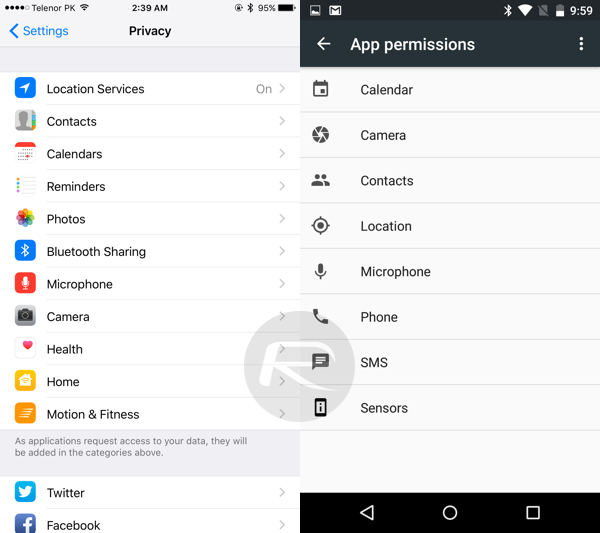
\includegraphics[height=0.5\linewidth]{media/graphics/ios-9-vs-android_privacy.png}

%\begin{columns}[T] % contents are top vertically aligned
%	\begin{column}[T]{5cm} % each column can also be its own environment
%		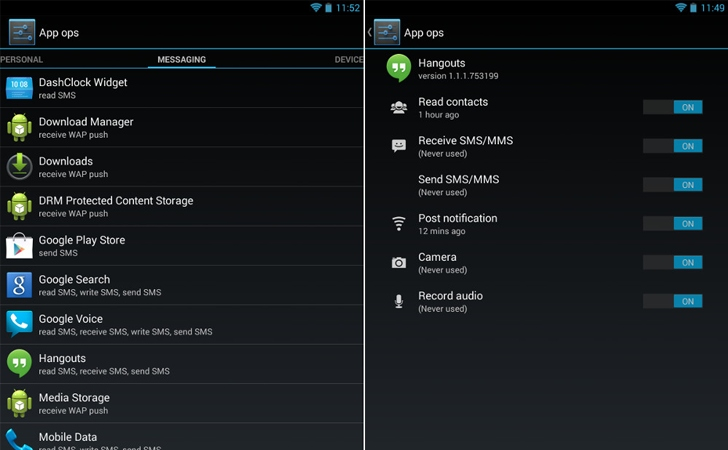
\includegraphics[height=3cm]{media/graphics/appops-android.jpg}
%	\end{column}
%	\begin{column}[T]{5cm} % alternative top-align that's better for graphics
%    	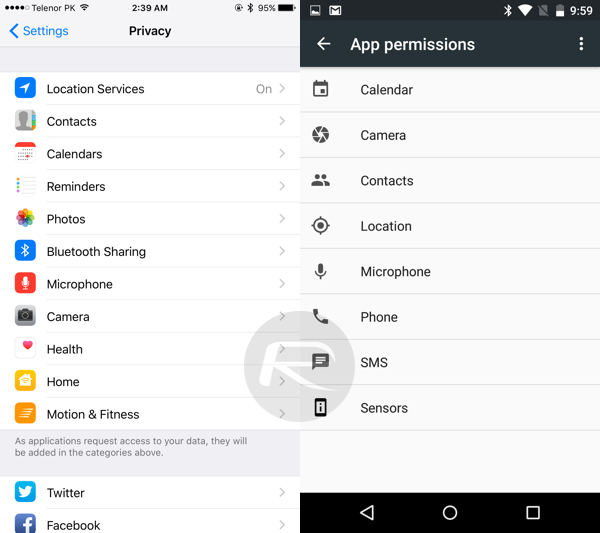
\includegraphics[height=3cm]{media/graphics/ios-9-vs-android_privacy.png}
%	\end{column}
%\end{columns}

\end{frame}
\end{document}
